\subsection{Nonlinear Dynamical Analysis}

Các cửa sổ ultra-short PPG hợp lệ được tái dựng trong không gian pha và khảo sát qua ba góc nhìn bổ sung. Simplex Projection đánh giá khả năng dự báo ở các horizon hữu hạn, RQA mô tả tổ chức tái diễn, còn Rosenstein LLE ước lượng phân kỳ quỹ đạo cục bộ. Các thuộc tính này không được quy về một thang mức độ chaos chung. Các metric được dùng trong kiểm định PPS để trả lời RQ1 và so sánh Awake--Drowsy để trả lời RQ2. Figure~\ref{fig:ntsa_framework} tóm tắt quy trình phân tích.

\begin{figure*}[t]
    \centering
    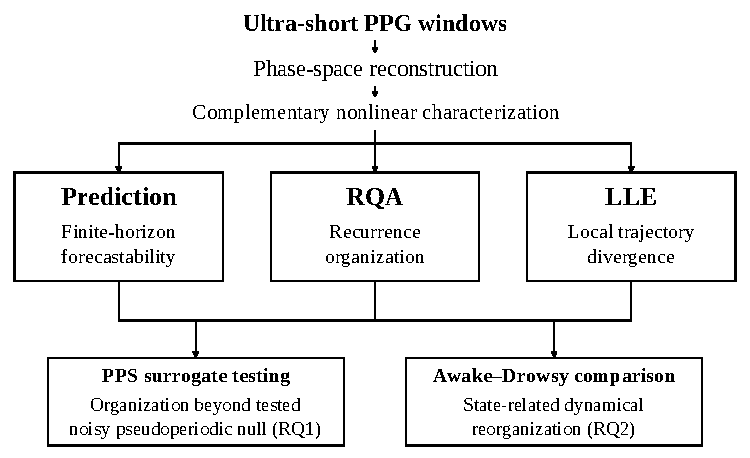
\includegraphics[width=0.82\textwidth]{manuscript/figures/ntsa_framework_overview.pdf}
    \caption{Overview of the nonlinear dynamical analysis framework. Ultra-short PPG windows are reconstructed in phase space and characterized through three complementary views: finite-horizon forecastability (Prediction), recurrence organization (RQA), and local trajectory divergence (LLE). PPS surrogate testing addresses RQ1, whereas Awake--Drowsy comparison addresses RQ2.}
    \label{fig:ntsa_framework}
\end{figure*}

\subsubsection{Phase-Space Reconstruction}

PPG đã xử lý được tái dựng bằng time-delay embedding theo Takens \cite{takens1981}. Average Mutual Information (AMI) \cite{fraser1986, ksg2004} và False Nearest Neighbors (FNN) \cite{kennel1992} hỗ trợ chọn delay $\tau$ và dimension $m$ (Figure~\ref{fig:phase_space_reconstruction}). Cấu hình $\tau=0.16$~s, $m=8$ được cố định chung cho Awake và Drowsy, không chọn theo hiệu ứng trạng thái hoặc p-value; delay được quy đổi thành $\tau_{\mathrm{samples}}=\mathrm{round}(\tau f_s)$, tương ứng 4/8 mẫu tại 25/50~Hz. Vector trạng thái được viết:

\begin{equation}
\mathbf{x}_i =
\left[
x_i,\,
x_{i-\tau},\,
x_{i-2\tau},\,
\ldots,\,
x_{i-(m-1)\tau}
\right],
\label{eq:time_delay_embedding}
\end{equation}

\begin{figure*}[t]
    \centering

    % =========================
    % Top row: A, B, C
    % =========================

    % Panel A
    \begin{minipage}[t]{0.32\textwidth}
        \centering
        \includegraphics[width=\linewidth]
        {image/phase_space_reconstruction/phase_space_ami_60s_processed.pdf}

        \vspace{0.25em}
        \small
        (A) AMI-based selection of the embedding delay $\tau$.
    \end{minipage}
    \hfill
    % Panel B
    \begin{minipage}[t]{0.32\textwidth}
        \centering
        \includegraphics[width=\linewidth]
        {image/phase_space_reconstruction/phase_space_fnn_60s_processed_awake.pdf}

        \vspace{0.25em}
        \small
        (B) FNN analysis for the Awake state.
    \end{minipage}
    \hfill
    % Panel C
    \begin{minipage}[t]{0.32\textwidth}
        \centering
        \includegraphics[width=\linewidth]
        {image/phase_space_reconstruction/phase_space_fnn_60s_processed_drowsy.pdf}

        \vspace{0.25em}
        \small
        (C) FNN analysis for the Drowsy state.
    \end{minipage}

    \vspace{0.8em}

    % =========================
    % Bottom row: D, E
    % =========================

    % Panel D
    \begin{minipage}[t]{0.40\textwidth}
        \centering
        \includegraphics[width=\linewidth]
        {image/phase_space_reconstruction/phase_space_reconstruction_awake.pdf}

        \vspace{0.25em}
        \small
        (D) Representative three-dimensional reconstructed state space for Awake.
    \end{minipage}
    \hspace{0.06\textwidth}
    % Panel E
    \begin{minipage}[t]{0.40\textwidth}
        \centering
        \includegraphics[width=\linewidth]
        {image/phase_space_reconstruction/phase_space_reconstruction_drowsy.pdf}

        \vspace{0.25em}
        \small
        (E) Representative three-dimensional reconstructed state space for Drowsy.
    \end{minipage}

    \caption{
    Phase-space reconstruction of the PPG signal.
    (A) Average Mutual Information (AMI) was used to determine the embedding delay, leading to the common choice $\tau=0.16$ s.
    (B--C) False Nearest Neighbors (FNN) analysis for the Awake and Drowsy states, respectively, with $m=8$ selected after the proportion of false neighbors reached a low plateau.
    (D--E) Representative three-dimensional projections of the reconstructed state space for Awake and Drowsy using the selected embedding parameters.
    The same reconstruction configuration, $\tau=0.16$ s and $m=8$, was fixed for all subsequent nonlinear time-series analyses.
    }
    \label{fig:phase_space_reconstruction}
\end{figure*}

\subsubsection{Simplex Projection}

Simplex Projection \cite{sugihara1990nonlinear} sử dụng cùng embedding $m=8$, $\tau=0.16$~s trên PPG đã xử lý. Dự báo leave-one-out dùng $k=m+1=9$ láng giềng Euclidean gần nhất của trạng thái $\mathbf{x}_t$, với khoảng cách thời gian lớn hơn 1.0~s. Trọng số theo khoảng cách được chuẩn hóa:

\begin{equation}
w_j =
\frac{
\exp\left(-d_j/d_1\right)
}{
\displaystyle\sum_{k=1}^{m+1}
\exp\left(-d_k/d_1\right)
},
\label{eq:simplex_weights}
\end{equation}

với $d_j$ là khoảng cách tới láng giềng thứ $j$ và $d_1$ là khoảng cách nhỏ nhất. Dự báo tại horizon $T_p$ là

\begin{equation}
\hat{x}_{t+T_p}
=
\sum_{j=1}^{m+1}
w_j x_{v_j+T_p},
\label{eq:simplex_prediction}
\end{equation}

trong đó $v_j$ là chỉ số thời gian của láng giềng thứ $j$. Dự báo dùng 18 horizons cố định từ 0.04 đến 4.00~s, quy đổi bằng $\mathrm{round}(T_p f_s)$; danh sách đầy đủ nằm trong Supplementary. Tại mỗi horizon của từng cửa sổ, Pearson CC và NRMSE được tính như sau:

\begin{equation}
    \mathrm{CC} =
    \frac{
    \sum_{i=1}^{N}
    \left(y_i-\bar{y}\right)
    \left(\hat{y}_i-\bar{\hat{y}}\right)
    }
    {
    \sqrt{
    \sum_{i=1}^{N}\left(y_i-\bar{y}\right)^2
    }
    \sqrt{
    \sum_{i=1}^{N}\left(\hat{y}_i-\bar{\hat{y}}\right)^2
    }
    },
    \label{eq:cc}
\end{equation}

\begin{equation}
    \mathrm{NRMSE} =
    \frac{
    \sqrt{
    \frac{1}{N}
    \sum_{i=1}^{N}
    \left(y_i-\hat{y}_i\right)^2
    }
    }
    {\sigma_y},
    \label{eq:nrmse}
\end{equation}

Ở đây, $y_i$ và $\hat{y}_i$ là giá trị quan sát và dự báo; $\bar{y}$ và $\bar{\hat{y}}$ là trung bình tương ứng; $N$ là số cặp quan sát--dự báo và $\sigma_y$ là SD của tín hiệu trong cửa sổ. CC cao hơn và NRMSE thấp hơn biểu thị khả năng dự báo cao hơn. Lấy mean của từng metric qua 18 horizons trong mỗi cửa sổ để thu window-level Mean CC và Mean NRMSE, sau đó lấy median qua các cửa sổ hợp lệ trong từng recording session $\times$ state. Figure~\ref{fig:simplex_example} minh họa một dự báo đại diện.

\begin{figure}[t]
    \centering
    \includegraphics[width=\columnwidth]{image/nonlinear_prediction/simplex_session_1_60s_processed_awake_window_1.pdf}
    \caption{
    Minh họa Simplex Projection trên một cửa sổ PPG đại diện.
    Tín hiệu quan sát được so sánh với tín hiệu dự báo tại một prediction horizon xác định trong không gian trạng thái tái dựng với $\tau=0.16$ s và $m=8$.
    Sự tương đồng giữa hai chuỗi được định lượng bằng CC, trong khi sai số dự báo được định lượng bằng NRMSE.
    }
    \label{fig:simplex_example}
\end{figure}

\subsubsection{Recurrence Quantification Analysis}

RQA mô tả tổ chức tái diễn của quỹ đạo trong cùng không gian tái dựng \cite{eckmann1987,marwan2007}. Recurrence matrix được xác định bởi

\begin{equation}
    R_{i,j}
    =
    \Theta
    \left(
    \varepsilon
    -
    \left\|
    \mathbf{x}_i-\mathbf{x}_j
    \right\|
    \right),
    \label{eq:recurrence_matrix}
\end{equation}

với $\Theta$ là hàm Heaviside và $\|\cdot\|$ là khoảng cách Euclidean. Ngưỡng $\varepsilon$ được chọn riêng từng cửa sổ với recurrence rate mục tiêu RR $=0.02$. Loại line of identity và các cặp có $|i-j|\leq W$, với Theiler window $W=(m-1)\tau_{\mathrm{samples}}$; độ dài đường tối thiểu là $l_{\min}=v_{\min}=2$. DET và $L_{\mathrm{mean}}$ mô tả tổ chức đường chéo, còn LAM và TT mô tả tổ chức thẳng đứng/laminar \cite{webber1994,marwan2002,marwan2007}.

Gọi $P(l)$ là số đường chéo có độ dài $l$. DET là tỷ lệ recurrence points thuộc các đường chéo đạt độ dài tối thiểu $l_{\min}$ \cite{webber1994,marwan2007}:

\begin{equation}
    \mathrm{DET}
    =
    \frac{
    \displaystyle
    \sum_{l=l_{\min}}^{N}
    lP(l)
    }
    {
    \displaystyle
    \sum_{l=1}^{N}
    lP(l)
    }.
    \label{eq:det}
\end{equation}

Độ dài trung bình của các đường chéo này là $L_{\mathrm{mean}}$ \cite{webber1994,marwan2007}:

\begin{equation}
    L_{\mathrm{mean}}
    =
    \frac{
    \displaystyle
    \sum_{l=l_{\min}}^{N}
    lP(l)
    }
    {
    \displaystyle
    \sum_{l=l_{\min}}^{N}
    P(l)
    }.
    \label{eq:lmean}
\end{equation}

Tương tự, với $P(v)$ là số đường thẳng đứng có độ dài $v$, LAM là tỷ lệ recurrence points thuộc các đường đạt độ dài tối thiểu $v_{\min}$ \cite{marwan2002,marwan2007}:

\begin{equation}
    \mathrm{LAM}
    =
    \frac{
    \displaystyle
    \sum_{v=v_{\min}}^{N}
    vP(v)
    }
    {
    \displaystyle
    \sum_{v=1}^{N}
    vP(v)
    }.
    \label{eq:lam}
\end{equation}

TT là độ dài trung bình của các đường thẳng đứng này \cite{marwan2002,marwan2007}:

\begin{equation}
    \mathrm{TT}
    =
    \frac{
    \displaystyle
    \sum_{v=v_{\min}}^{N}
    vP(v)
    }
    {
    \displaystyle
    \sum_{v=v_{\min}}^{N}
    P(v)
    }.
    \label{eq:tt}
\end{equation}

Bốn metric được tính trên từng cửa sổ hợp lệ (Figure~\ref{fig:rqa_example}). DET mô tả tổ chức tái diễn theo đường chéo, không đồng nhất với tính tất định vật lý.

\begin{figure*}[t]
    \centering
    \includegraphics[width=0.82\textwidth]{image/rqa/recurrence_plot_session_1_60s_processed.pdf}
    \caption{
    Recurrence plots đại diện của PPG trong hai trạng thái Awake và Drowsy.
    Các cấu trúc đường chéo được định lượng bằng DET và $L_{\mathrm{mean}}$, trong khi các cấu trúc thẳng đứng được định lượng bằng LAM và TT.
    Figure này minh họa hình học recurrence của tín hiệu PPG; các so sánh định lượng giữa hai trạng thái được thực hiện trên các metric RQA tính tại từng cửa sổ.
    }
    \label{fig:rqa_example}
\end{figure*}

\subsubsection{Largest Lyapunov Exponent}

Rosenstein LLE \cite{rosenstein1993} theo dõi sự phân kỳ của các cặp trạng thái lân cận trong cùng embedding $m=8$, $\tau=0.16$~s. Mỗi trạng thái được ghép với một láng giềng Euclidean gần nhất có khoảng cách thời gian lớn hơn Theiler window, xác định bằng spectral mean period của từng cửa sổ. Với khoảng cách ban đầu $d_j(0)$ và bước lấy mẫu $\Delta t=1/f_s$, quan hệ phân kỳ được viết

\begin{equation}
    d_j(i) \approx d_j(0)e^{\lambda_1 i\Delta t},
    \label{eq:lle_divergence}
\end{equation}

Lấy logarit và trung bình trên các cặp láng giềng thu được

\begin{equation}
    y(i) =
    \frac{1}{\Delta t}
    \left\langle
    \ln d_j(i)
    \right\rangle
    \approx
    \frac{1}{\Delta t}
    \left\langle
    \ln d_j(0)
    \right\rangle
    + \lambda_1 i,
    \label{eq:lle_mean_log_divergence}
\end{equation}

với $\langle\cdot\rangle$ là trung bình theo $j$; hệ số góc của vùng tuyến tính ước lượng $\lambda_1$, đơn vị $\mathrm{s}^{-1}$. Theo dõi tối đa 5.0~s và fit trong khoảng 0.80--1.30~s, với tối thiểu 50 cặp ban đầu, 30 cặp tại mỗi điểm fit và ba điểm fit. Chấp nhận fit hữu hạn có $R^2\geq0.90$ (Figure~\ref{fig:lle_example}). LLE mô tả phân kỳ quỹ đạo cục bộ trên dữ liệu hữu hạn, không chứng minh deterministic chaos.

\begin{figure}[t]
    \centering
    \includegraphics[width=\columnwidth]{image/lle/lle_session_1_60s_processed_awake_window_1.pdf}
    \caption{
    Minh họa ước lượng largest Lyapunov exponent bằng phương pháp Rosenstein.
    Đường cong biểu diễn phân kỳ trung bình logarit theo thời gian tiến hóa, trong khi đoạn gạch đứt biểu thị vùng fit tuyến tính được dùng để ước lượng hệ số góc tương ứng với LLE.
    }
    \label{fig:lle_example}
\end{figure}

\subsubsection{Pseudoperiodic Surrogate Testing}

PPS theo Small \textit{et al.} \cite{small2001} cung cấp noisy pseudoperiodic null phù hợp với cấu trúc dao động gần chu kỳ của PPG. Sau tái dựng, surrogate được sinh qua các bước chuyển xác suất giữa các trạng thái lân cận:

\begin{equation}
    P\left(\mathbf{s}_j=\mathbf{z}_t \mid \mathbf{s}_i\right)
    \propto
    \exp\left(
    -\frac{
    \left\|\mathbf{z}_t-\mathbf{s}_i\right\|
    }{\rho}
    \right),
    \label{eq:pps_transition_probability}
\end{equation}

trong đó $\rho$ điều chỉnh mức ưu tiên các trạng thái gần nhau. PPS giữ cấu trúc pseudoperiodic tổng quát nhưng thay đổi tiến triển quỹ đạo cục bộ (Figure~\ref{fig:pps_example}). Để trả lời RQ1, mỗi cửa sổ gốc hợp lệ được so với 39 surrogates trên bảy metric: CC, NRMSE, DET, $L_{\mathrm{mean}}$, LAM, TT và LLE, dùng cùng cấu hình ước lượng. Bác bỏ null cho thấy tổ chức quan sát được không được tái tạo đầy đủ bởi noisy pseudoperiodic null đã kiểm tra; kết quả này không chứng minh deterministic chaos hoặc loại trừ mọi giải thích ngẫu nhiên.

\begin{figure}[t]
    \centering
    \includegraphics[width=\columnwidth]{image/pps/pps_visual_sanity_check_session_01_60s_window_0_15s_processed.pdf}
    \caption{
    Minh họa một cửa sổ PPG đã xử lý và một pseudoperiodic surrogate tương ứng.
    PPS duy trì đặc tính dao động gần chu kỳ của tín hiệu PPG nhưng thay đổi sự tiến triển cục bộ của quỹ đạo thông qua các bước chuyển xác suất trong không gian trạng thái.
    Surrogate được sử dụng làm noisy pseudoperiodic null model cho kiểm định RQ1.
    }
    \label{fig:pps_example}
\end{figure}

\subsection{Statistical and Sensitivity Analysis}

Cửa sổ hợp lệ là đơn vị tính toán, còn recording session là đơn vị suy luận cho RQ2. Mỗi metric được tổng hợp bằng median qua các cửa sổ hợp lệ trong session $\times$ state; Mean CC/Mean NRMSE được tính sau bước lấy mean qua horizons trong từng cửa sổ. Trên 20 recording sessions, tính chênh lệch ghép cặp $\Delta_i=\mathrm{Drowsy}_i-\mathrm{Awake}_i$ và báo cáo median paired $\Delta$, p-value của Wilcoxon signed-rank hai phía, matched-pairs rank-biserial correlation $r_{\mathrm{rb}}$ và percentile bootstrap 95\% CI của median với 20,000 lần lấy mẫu lại theo paired-session. Benjamini--Hochberg FDR được áp dụng một lần trên đúng bảy metric nominal 60~s: Mean CC, Mean NRMSE, DET, $L_{\mathrm{mean}}$, LAM, TT và LLE; ngưỡng hỗ trợ thống kê là $q_{\mathrm{BH}}<0.05$.

Đối với RQ1, giá trị gốc được xếp hạng cùng $M=39$ surrogates trong tập 40 giá trị. Với hạng $r$, p-value của finite-sample rank test hai phía là
\begin{equation}
p=\min\left(1,\frac{2\min(r,M+2-r)}{M+1}\right).
\label{eq:pps_rank_test}
\end{equation}
Với $M=39$, $p_{\min}=0.05$ và bác bỏ null khi $p\leq0.05$. Kiểm định thực hiện ở cấp cửa sổ; tỷ lệ bác bỏ tổng hợp qua cửa sổ và sessions là thống kê mô tả, không phải kiểm định ghép cặp của RQ2.

Độ nhạy được khảo sát theo độ dài cửa sổ 30/60/120/180~s, định nghĩa nhãn T30/T60/S3/S5, tham số tái dựng và ước lượng, cùng unknown repeated-session dependence. Do không có liên kết participant--session, độ nhạy với sự phụ thuộc này được khảo sát dưới các hypothetical two-session clusters; phân tích không xác lập suy luận cấp participant. Các cấu hình kiểm tra, quy tắc nhãn và phương pháp clustering được trình bày trong Supplementary.
